\famichapter{Development Process}{This chapter documents how FamiPet was
developed: the workflow rules, the phase-based roadmap, and the project
timeline reconstructed from the repository history.}{ch:process}

\section{Development Workflow}

The project follows the workflow encoded in \texttt{AGENTS.md}: inspect before
changing, treat the backend as the source of truth for identity and ownership,
preserve existing functionality, use real data only, persist through the
database, enforce security on the backend, make the smallest correct change,
test the complete flow, and never claim unverified results. Each phase of work
is completed as an atomic unit: inspect, implement, test, fix failures, update
documentation, commit, tag and push when specified, verify a clean working
tree, and stop.

Every change must reuse existing models, routes, controllers, and utilities
instead of duplicating endpoints or bypassing authentication. The role and
ownership of every resource are enforced on the backend, never by hiding UI
controls. The disciplined, phase-based engineering practices follow the
software-engineering fundamentals collected by~\cite{sommerville}.

\section{Phase-Based Roadmap}

The implementation is tracked in \texttt{ROADMAP.md} as numbered phases. The
frontend phase status below is taken directly from the roadmap. Each
implemented phase is delivered as an atomic commit; the \emph{Commit} column
records the feature commit that completes the phase.

\begin{center}
\begin{longtable}{@{}p{1.2cm}p{5.4cm}p{1.6cm}p{3.4cm}@{}}
\caption{Roadmap phase status.}
\label{tab:phases}\\
\toprule
\textbf{Phase} & \textbf{Name} & \textbf{Status} & \textbf{Commit} \\
\midrule
1 & Scaffold (Vite + React + TS) & Complete & \texttt{80cc21d} \\
2 & Tailwind setup & Complete & \texttt{80cc21d} \\
3 & Assets and theme & Complete & \texttt{80cc21d} \\
4 & Routing & Complete & \texttt{c5f23f3} \\
5 & Global styles and shared layout & Complete & \texttt{be87712} \\
6 & Shared layout components & Complete & \texttt{1a2cf5e} \\
7 & Authentication & Complete & \texttt{9b44727} \\
8 & Dashboard & Complete & \texttt{d2f6952} \\
9 & Pet management & Complete & \texttt{38c6aa9} \\
10 & Health & Complete & \texttt{17fc630} \\
11 & Vaccinations & Complete & \texttt{3d10701} \\
12 & Appointments & Complete & \texttt{e003c98} \\
13 & Veterinarians & Complete & \texttt{721f03f} \\
14 & Reminders & Complete & \texttt{56a1c29} \\
15 & Community & Complete & \texttt{5dd0fef} \\
16 & Lost \& found & Complete & \texttt{d637cd9} \\
17 & Favourites & Complete & \texttt{d7a6f10} \\
18 & Adoption & Complete & \texttt{70293d0} \\
19 & Pet breeds & Complete & \texttt{526f78e} \\
20 & Settings & Complete & \texttt{ed4d6cb} \\
21 & Admin panel & Complete & \texttt{d18c336} \\
22 & AI / PetGPT frontend & Complete & \texttt{d26e955} \\
23 & API integration layer & Planned & --- \\
24 & Auth / state consolidation & Planned & --- \\
25 & UI/UX completion & Planned & --- \\
26 & Visual regression & Planned & --- \\
27 & Functional regression & Planned & --- \\
28 & Docker / Nginx integration & Planned & --- \\
29 & Client consolidation & Planned & --- \\
\bottomrule
\end{longtable}
\end{center}

\section{Timeline and Project Gantt}

The project was initiated in July 2026. The initial period (July and August)
covered planning, requirements analysis, and design, and is recorded in the
project documentation; the repository itself does not carry those commits. The
version-controlled implementation begins on 2026-09-07 with the backend
commits. The Step-10 verification campaign was executed on 2026-09-09, and the
React frontend phases were implemented from 2026-09-21 through 2026-09-22,
with phases 23--29 still planned. The roadmap does not record dates, so the
timeline below is reconstructed from the repository history and the documented
project start, following the scheduling conventions of the
PMBOK~\cite{pmbok}; the Gantt chart itself was rendered with
Mermaid~\cite{mermaid}.

\begin{figure}[htbp]
    \centering
    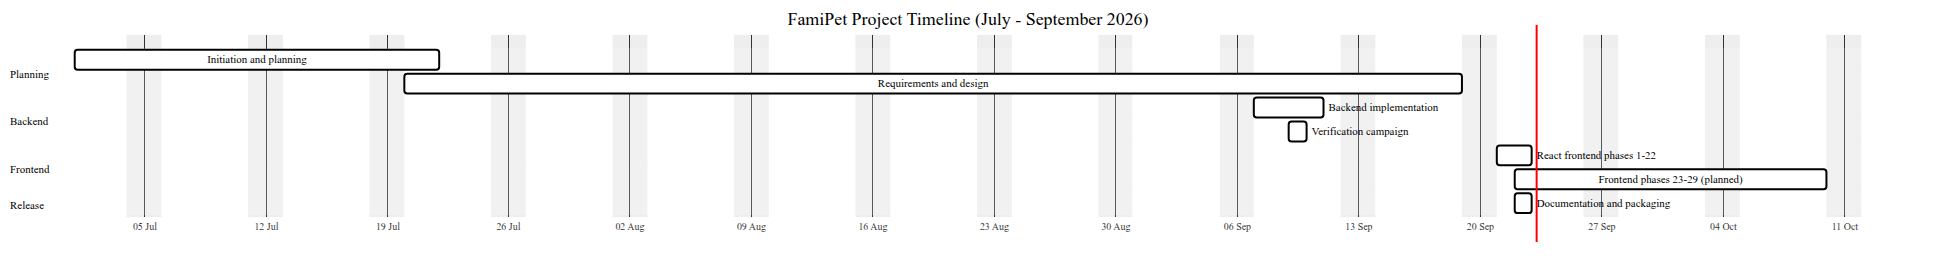
\includegraphics[width=\textwidth]{figures/19-project-gantt.png}
    \caption{Project timeline and Gantt chart (July--September 2026).}
    \label{fig:gantt}
\end{figure}

The key milestones are summarised in Table~\ref{tab:milestones}.

\begin{center}
\begin{longtable}{@{}p{4.2cm}p{3.2cm}p{7.2cm}@{}}
\caption{Key project milestones.}
\label{tab:milestones}\\
\toprule
\textbf{Activity} & \textbf{Period} & \textbf{Evidence} \\
\midrule
Initiation and planning & Jul 2026 & Project brief and design direction. \\
Requirements and design & Jul--Aug 2026 & Requirements, architecture, and
design documentation. \\
Backend implementation & 07--10 Sep 2026 & Initial commits; the sixteen route
modules covering all documented features. \\
Verification campaign & 09 Sep 2026 & \texttt{Step10-Report.md}: browser sweep,
persistence, admin, and security tests. \\
React frontend phases 1--22 & 21--22 Sep 2026 & Roadmap phase table
(Table~\ref{tab:phases}) with commit hashes. \\
Documentation and packaging & 22 Sep 2026 & Black book, project skills, and
graphify artifacts committed. \\
\bottomrule
\end{longtable}
\end{center}